% One-sided document
\documentclass[12pt, oneside]{ociamthesis}
\usepackage{helvet}
\usepackage{amssymb}
\usepackage[utf8]{inputenc}
\usepackage[T1]{polski}
\usepackage{url}
\usepackage[hidelinks]{hyperref}
\usepackage[table,xcdraw]{xcolor}
\usepackage[leftbars]{changebar}
\hypersetup{
	pdftitle={Metaanaliza użyteczności zbiorów danych do zastosowań w~uczeniu maszynowym},
	pdfsubject={Praca licencjacka},
	pdfauthor={Mateusz Piotr Moruś},
	pdfkeywords={metaanaliza, zbiory danych, uczenie maszynowe, web-scraping}
}
\usepackage{graphicx}
\usepackage{listings}
\usepackage{xcolor}

\definecolor{codegreen}{rgb}{0,0.6,0}
\definecolor{codegray}{rgb}{0.5,0.5,0.5}
\definecolor{backcolour}{rgb}{0.95,0.95,0.92}

\lstdefinestyle{mystyle}{
    backgroundcolor=\color{backcolour},
    commentstyle=\color{codegreen},
    keywordstyle=\color{magenta},
    numberstyle=\tiny\color{codegray},
    stringstyle=\color{codegreen},
    basicstyle=\ttfamily\footnotesize,
    breakatwhitespace=false,
    breaklines=true,
    captionpos=b,
    keepspaces=true,
    numbers=left,
    numbersep=5pt,
    showspaces=false,
    showstringspaces=false,
    showtabs=false,
    tabsize=4
}

\lstset{style=mystyle}


\setlength{\changebarsep}{-5em}

\graphicspath{ {./Images/} }
\AtBeginDocument{\let\textlabel\label}

% Make the numbering of figures continuous
\counterwithout{figure}{chapter}
% Make the numbering of tables continuous
\counterwithout{table}{chapter}

\title{Metaanaliza użyteczności zbiorów danych do zastosowań w~uczeniu maszynowym}
\engtitle{Meta-analysis of the utility of data sets for applications in machine learning}
\author{Mateusz Piotr Moruś}
\albumnumber{292540}
\university{UNIWERSYTET MARII CURIE-SKŁODOWSKIEJ W~LUBLINIE}
\college{Wydział Matematyki, Fizyki i~Informatyki}
\field{Informatyka}
\speciality{-}
\submittedtext{Praca licencjacka}
\department{Katedrze Neuroinformatyki i~Inżynierii Biomedycznej}
\promoter{dr. hab. Grzegorza Marcina Wójcika, prof. UMCS}
\degreedate{Lublin rok 2021}

\begin{document}

% This baselineskip gives sufficient line spacing for an examiner to easily markup the thesis with comments
\baselineskip=18pt plus1pt

% Set the number of sectioning levels that get number and appear in the contents
\setcounter{secnumdepth}{3}
\setcounter{tocdepth}{3}

% Add a title page
\maketitle

% Add an abstract
\begin{abstract}
	Rozwój dziedziny uczenia maszynowego pozwolił na rozwiązywanie problemów dotychczas nieosiągalnych tradycyjnym metodom badawczym.
	Jakość takiego uczenia często jednak zależy od danych użytych w~procesie.
	Jakość danych jest tematem, który się często pojawia i~jest powszechnie uważana za istotny element ogólnie pojętego przetwarzania danych, jednak nie ma wyprowadzonego i~dobrze zbadanego sposobu jej określenia czy powiedzenia, na czym ta jakość tak na prawdę polega.
	Syntaktyczne cechy zbiorów danych, które mogą pozwolić na analizę jakości danych z~praktycznej strony, mogą być uchwycone i~reprezentowane w~postaci metadanych.
	Dotychczasowe prace badawcze analizowały metadane w~kontekście problemów z~nimi związanych, stosowalności algorytmów kategoryzujących oraz próby określenia ontologii jakości zbiorów danych.
	W tej pracy podejmuję metaanalizę badając zależności między metadanymi dotyczącymi cech zbiorów a~ich użytecznością i~atrakcyjnością użytkową.
	Badam stosowne korelacje oraz próbuję odnaleźć, czy istnieją powiązania między przynależnością do pewnych kategorii syntaktycznych a~popularnością zbioru i~jakie są to prawidłowości.
	Sugeruję również sposób, w~jaki można przetestować i~doprecyzować rezultaty mojego badania w~przyszłych pracach.
\end{abstract}

% Add an abstract in english
\begin{abstract-en}
	The development of the field of machine learning has allowed us to solve problems unattainable by traditional research methods up to this point.
	However, the quality of such learning often depends on the data used in the process.
	Data quality is a~topic that arises fairly often and is widely regarded as an essential element of data processing in general, but there is no clear and well-researched way of describing it or determining what that quality really is.
	The syntactic characteristics of datasets that can allow data quality analysis from a~practical side of view can be captured and represented in the form of metadata.
	Previous research has analysed metadata in the context of problems related to it, the applicability of categorization algorithms and attempts to state the ontology of dataset quality.
	In this work, I~undertake a~meta-analysis examining the relationship between metadata describing characteristics of collections and their utility and functional attractiveness.
	I am investigating the relevant correlations and trying to figure out whether there are links between belonging to certain syntactic categories and the popularity of the collection and what those regularities are.
	I also suggest how to test and refine my results in future studies.
\end{abstract-en}


% Start roman page numbering
\begin{romanpages}
	% Generate and include a table of contents
	\tableofcontents
	% Create a group for list of figures and list of tables to fit both on one page
	\begingroup
	\let\clearpage\relax
	% Generate and include a list of figures
	\listoffigures
	% Generate and include a list of tables
	\listoftables
	\endgroup
% End roman page numbering
\end{romanpages}

% Include the introduction
% Analiza danych o otaczającym nas świecie jest jedną z kluczowych metod postępu, zarówno naukowego jak i technologicznego.
% Skuteczność takiej analizy jest jednak zależna od jakości dostępnych danych.

% Problem z nieustrukturyzowanymi danymi zauważalny był jeszcze długo zanim ilości generowanych danych sięgały ułamka dzisiejszego natłoku informacji \cite{blumberg2003problem}, a wraz z czasem problem ten się tylko nasila.
% Aby móc skutecznie wnioskować z użyciem danego zbioru informacji powinien on być ustrukturyzowany.
% Najpowszechniejszym przykładem ustrukturyzowania są zbiory danych (\textit{datasets}), najczęściej w postaci tabelarycznej.
% Często używane jest pojęcie \textit{baz danych} zamiennie ze zbiorami danych, jednak nie jest to prawidłowe.
% Bazy danych to kontenery zawierające zarówno zbiory danych, jak i całą infrastrukturę służącą do interakcji i manipulacji danymi znajdującymi się wewnątrz.
% Zawartych zbiorów często jest więcej niż jeden i są powiązane relacyjnie między sobą.
% Istnieją archiwa przechowujące tego typu ustrukturyzowane zbiory danych i udostępniające je publicznie do wykorzystania najczęściej do celów badawczych.
% Jedno z nich to UC Irvin Machine Learning Repository (\url{https://archive.ics.uci.edu/}), gdzie poza samymi zbiorami danych znajdują się na ich metadane.

% Metadane zbioru danych to cechy opisujące sam zbiór, takie jak ilość rekordów (krotek, wierszy) czy atrybutów (kolumn).
% Oczywistym jest, że w użyteczności danego zbioru najistotniejsza jest jego semantyka, informacje w nim zawarte.
% Jednak syntaktyka również odgrywa swoją rolę; jednym z bardziej oczywistych przykładów może być ilość danych.
% W zdecydowanej większości im więcej danych zawartych jest w zbiorze tym lepiej, chociaż i od tej reguły pojawiają się wyjątki \cite{gasco2012does,boivin2006more}.
% Na jakość zbioru wpływ ma także obecność brakujących danych, mimo istnienia algorytmów pozwalających na ich uzupełnienie \cite{acuna2004treatment}.

% W tej pracy przeanalizuję metadane zbiorów danych i ich wpływ na popularność i użyteczność zbioru.
% Przedstawię również projekt badawczy analogiczny do mojego pozwalający na dokładniejszą i rozszerzoną metaanalizę, aby docelowo odnaleźć zależności syntaktyczne i pomóc w tworzeniu zbiorów danych bogatszych i łatwiejszych w analizie.

\chapter*{Wstęp}
\addcontentsline{toc}{chapter}{Wstęp}
\label{ch:introduction}

Uczenie maszynowe jest fantastycznym narzędziem pozwalającym na wykonywanie zadań dotychczas niedostępnych tradycyjnym algorytmom poprzez wykorzystanie kluczowej zdolności uczenia się i samo-ulepszenia.
Trzema najważniejszymi jego zastosowaniami są programy samo-przystosowujące, aplikacje, których nie można zaprogramować ręcznie ze względu na ich złożoność oraz użycie danych historycznych w celu ulepszenia przewidywania i podejmowania decyzji \cite{mitchell1997machine}.
Żadne z tych zastosowań nie byłoby jednak możliwe bez dostępności odpowiednich danych.

Dane i zbiory danych są kluczowym elementem systemów uczenia maszynowego.
Potrzebne w konkretnym zastosowaniu dane można wygenerować lub zebrać osobiście, jednak istnieją dedykowane repozytoria pozwalające na wyszukanie i wykorzystanie interesujących zbiorów danych oraz dotację tych przez nas zebranych.
Taka ogólnodostępność pozwala na wielokrotne użycie tych samych danych w różnych zastosowaniach lub przez różne osoby.
Jako przykład można podać znany wielu osobom zbiór odręcznie zapisanych cyfr MNIST \cite{mnist}.
Autorzy zbioru zadbali o jego jakość, znormalizowali wielkość obecnych tam cyfr, zastosowali antyaliasing oraz wycentrowali powstałe obrazki względem ich środka ciężkości.
Zabieg ten był niezwykle istotny, ponieważ pośrednio wpłynął na jakość wszystkich badań i analiz prowadzonych z użyciem tego zbioru danych.

Obrazuje to wagę, jaką powinno się przykładać do utrzymania jakości zbiorów danych.
Ma tutaj bowiem zastosowanie popularna w informatyce zasada \textit{śmieci na wejściu - śmieci na wyjściu} (ang. \textit{"garbage in -- garbage out"}).
Mówi ona, że nawet w przypadku idealnej logiki programu, podanie na wejściu niepoprawnych danych wygeneruje niepoprawne wyniki.
W tym kontekście uczenie systemu z wykorzystaniem danych o niskiej jakości spowoduje, że rezultaty generowane przez ten system również będą niskiej jakości, nieprecyzyjne czy po prostu niepoprawne.

Przez taką jakość można rozumieć semantyczną zawartość zbioru, gdzie obecność błędnych danych w sposób oczywisty wpływa na działanie systemu.
Jednak często pomijana jest \textit{syntaktyka zbioru danych}, czyli sposób ustrukturyzowania czy reprezentacji zawartych danych.
Zmiany wprowadzone do zbioru MNIST przez jego autorów można, przynajmniej częściowo, uznać za zmiany tego właśnie typu.
Powstaje pytanie jakie z tych wartości syntaktycznych mają wpływ na jakość zbioru oraz w jaki sposób na niego oddziałują.
Niektóre z nich, takie jak właśnie ilość zawartych rekordów czy obecność brakujących danych wydają się mieć oczywisty wpływ.
Można się jednak zastanowić nad innymi, jak rodzaj zawartych danych czy ilość atrybutów.
W kontekście zbiorów danych ich syntaktyka może być reprezentowane przez ich \textit{metadane}.
Jeśli zbierzemy wszystkie te cechy w postaci metadanych, można przeprowadzić ich analizę w celu znalezienia zależności i powiązań.

Zależności między metadanymi a jakością i użytecznością ich zbiorów danych nie były dotychczas dobrze przebadane.
Obecnie jedyne dostępne metaanalizy opierające się na metadanych zbiorów, które zostały przeprowadzone, opierają się na innych kontekstach, takich jak aplikowalność algorytmów uczenia maszynowego \cite{brazdil1994characterizing}.

W tej pracy przeanalizuję metadane reprezentujące cechy i własności zbiorów danych zawartych w UC Irvin Machine Learning Repository \cite{Dua:2021}.
Dodatkowo przedstawię sposób pozyskania danych i skonstruowania zbioru przy braku publicznie dostępnego API oraz sposób analizy takich danych.
% Dostęp do upublicznionego zbioru i kodu Scrapera?

% Include the first chapter
\chapter{Metaanaliza i~analiza metadanych}

Metaanaliza oznacza wtórne odkrywanie wiedzy za pomocą uogólnienia informacji znajdujących się w~pierwotnych źródłach \cite{higgins2019cochrane}.
W przypadku tej pracy istotny jest aspekt metaanalizy polegający na \textit{analizie metadanych}, czyli przeprowadzeniu analizy z~użyciem standardowych narzędzi, ale na metadanych zbioru zamiast danych właściwych.
W rezultacie warto najpierw przyjrzeć się samej analizie danych.

\section{Analiza danych}

Otacza nas niemal nieskończony zasób informacji o~świecie.
Nawet biorąc pod uwagę jedynie dane cyfrowe IDC (\textit{International Data Corporation}) estymowała, że rocznie w~roku 2020 wytwarzanych będzie 35 zetabajtów danych \cite{tien2013big}.
Ilość ta została osiągnięta już dwa lata wcześniej; W~2018 pojawiały się wzmianki mówiące, że już wtedy roczna ilość wytwarzanych danych osiągnęła 33 zetabajty \cite{Patrizio:2018}, a~aktualnie IDC mówi o~nawet 59 zetabajtach \cite{IDC:2020}.
Mimo, że generowane są tak potężne zasoby danych, aby móc je wykorzystać trzeba do nich dotrzeć oraz odpowiednio przygotować.
Bez tego ich analiza staje się niezwykle trudna lub niemal niemożliwa.

	\subsection{Zdobywanie i~przetwarzanie danych}
	Sama obecność informacji w~środowisku nie jest wystarczająca aby móc je w~jakikolwiek sposób wykorzystać.
	Proces \textit{Data Science} składa się z~pięciu kroków, z~których pierwszym jest właśnie wydobycie danych.

	W nauce eksperymentalnej, w~tym nawet w~jej najświeższych gałęziach na początku fazy opisu jakościowego, badania zjawisk oparte są na pomiarach \cite{brandt1998data}.
	Dzisiaj wszelkie pomiary, zarówno w~nauce jak zastosowaniach praktycznych, są w~zdecydowanej większości rezultatem działania sensorów.
	Struktura i~sposób ich działania może być zróżnicowany i~złożony \cite{deshpande2004model,boyer2009scada}, ale cel jest jeden -- przechwycić interesujące nas dane o~świecie zewnętrznym.
	Działanie takich sensorów niestety często generuje dane nieustrukturyzowane, które sprawiają duży problem w~zarządzaniu i~są trudne do efektywnego przeanalizowania \cite{blumberg2003problem}.

	Z reguły dąży się, aby uzyskane dane doprowadzić do stanu jak najlepszej używalności i~przetwarzalności, a~co za tym idzie, aby w~jakiś sposób je ustrukturyzować.
	Istnieją bowiem techniki, które pozwalają na taką strukturyzację danych pierwotnie nieustrukturyzowanych, jedną z~nich jest zareprezentowanie danych i~ich schematu za pomocą grafów z~opisanymi krawędziami \cite{buneman1997adding}.
	Jeśli jednak ustrukturyzowanie danych nie jest możliwe, zostały zaproponowane techniki pozwalające na przynajmniej częściowe przeprowadzenie analizy danych nieustrukturyzowanych \cite{boulton1996analysis}.
	Często taka analiza prowadzi do utworzenia zbioru z~jej wynikami będącego zbiorem danych ustrukturyzowanym, który następnie wykorzystywany jest w~dalszych badaniach.

	\subsection{Analiza danych}

	Otrzymane i~przetworzone dane zawierają w~sobie potencjalną wartość, która jednak bez dalszej obróbki nie jest w~żaden sposób pożyteczna.
	Bardzo znana i~popularna piramida DIWM (dane, informacja, wiedza, mądrość) \cite{rowley2007wisdom}, nazywana także hierarchią wiedzy, dobrze obrazuje ten koncept.
	W tej piramidzie dane są najniższym stopniem, podstawą dla wszystkich pozostałych, najszersza ze względu na swój brak przetworzenia.
	Dane są definiowane jako ilościowy lub jakościowy zbiór symboli.
	Informacja natomiast to zbiór znaczących znaków, które mają możliwość wytworzenia wiedzy \cite{zins2007conceptual}.
	Idąc za tym konceptualnym podziałem, zbiory danych, które zostały poddane obróbce czy przetworzeniu zawierają nie tylko dane, ale także informacje.
	Poddanie takiego zbioru analizie można w~uproszczeniu opisać jako proces zamiany tej informacji w~wiedzę.
	W rzeczywistości, trzymając się modelu piramidy DIWM analiza będzie odpowiednikiem przetworzenia dużej ilości informacji w~mały podzbiór informacji, która będzie znacznie bogatsza znaczeniowo.
	Jednak biorąc pod uwagę, że z~samego założenia przetwarzania danych ten podzbiór ma docelowo być zinterpretowany i~zamieniony w~wiedzę, uproszczenie to nie odbiega bardzo od rzeczywistości.

	Można zdefiniować dwa główne rodzaje rozróżnienia analiz danych: analizy wyjaśniające/potwierdzające, a~także analizy deskryptywne/indukcyjne \cite{berthold2003intelligent}.
	Pierwsze rozróżnienie jest dość oczywiste.
	Analizę danych można przeprowadzać w~celu wyjaśnienia zaistnienia pewnego zjawiska lub aby potwierdzić jego istnienie.
	Drugie nie jest aż tak intuicyjne, chociaż nadal uzasadnione.
	Analizy deskryptywne, inaczej nazywane podsumowującymi mają na celu znalezienia prawidłowości i~cech o~całości zebranych danych, na przykład jaki jest odsetek kobiet w~populacji.
	Natomiast analizy indukcyjne próbują wyciągnąć wnioski generalizujące zaobserwowane trendy, na przykład jaki będzie prawdopodobny odsetek kobiet w~populacji w~przyszłym roku.
	Tego typu analiza jest szczególnie przydatna, kiedy nie ma dostępnych danych na temat całości populacji czy dziedziny danych zawartych w~zbiorze, co ma miejsce w~przeważającej części przypadków.
	Wtedy za pomocą analizy indukcyjnej wyciąga się wnioski generalizując tendencje podzbioru populacji czy dziedziny na cały zbiór.

\section{Metaanaliza}

	Analizowanie danych pozwala wyciągnąć wnioski na temat dziedziny, którą opisują.
	Metaanaliza natomiast pozwala na wyciągnięcie wniosków o~samym zbiorze danych, co często jest nieosiągalne w~inny sposób.
	Wyniki takiej analizy mogą być wysoce przydatne zarówno w~podejmowaniu decyzji na temat zbioru, jak również w~dalszych analizach, które dadzą już w~rezultacie informacje szersze, niż dotychczas było to możliwe.

	\subsection{Metadane}

	Metadane to dane, które dostarczają informacji na temat innych danych.
	Zobrazować to można wysłaniem wiadomości na portalu społecznościowym, który zapisuje w~serwisie nie tylko treść wiadomości, ale także inne informacje o~niej: datę i~godzinę wysłania, autora, adresata, status dostarczenia czy odczytania.

	Wyróżnia się cztery główne grupy określane jako metadane \cite{riley2017understanding}:

	\begin{itemize}
		\item Metadane opisowe (\emph{Descriptive metadata}) \\
		Informacje na temat zawartości zasobu służące jego lepszemu zrozumieniu.

		\item Metadane administracyjne (\emph{Administrative metadata}) \\
		Zawiera w~sobie metadane techniczne służące dekodowaniu czy renderowaniu zawartych danych, a~także metadane prawne do oznaczenia własności intelektualnej.

		\item Metadane strukturalne (\emph{Structural metadata}) \\
		Opisuje wzajemne relacje między częściami zasobu.

		\item Języki znacznikowe (\emph{Markup languages}) \\
		Języki mieszające zawartość oraz metadane w~całość.
		Przykładem takiego języka jest Markdown służący do pisania sformatowanego tekstu.
	\end{itemize}

	Wspomniane informacje o~wiadomości na portalu społecznościowym zaliczyć można do \emph{metadanych opisowych}.
	Z kolei treść zawarta w~tagu \lstinline{<meta charset="UTF-8">} używany w~języku HTML zaliczymy do \emph{metadanych technicznych}, służy bowiem rozpoznaniu kodowania, które powinno zostać użyte przy odczytywaniu zawartości.
	Co więcej, sam HTML podpada pod kategorię \emph{języka znacznikowego}.

	W odniesieniu do zbiorów danych metadanymi technicznymi będzie na przykład informacja, jaki jest używany separator: przecinek, tabulator czy inny, mniej popularny znak.
	Natomiast szerzej niż się pierwotnie wydaje można objąć termin \emph{metadanych opisowych}.
	Zaliczyć bowiem możemy tutaj informacje opisujące rodzaj danych zawartych w~zbiorze, jak i~samą jego strukturę.
	Do przykładów takich informacji możemy zaliczyć liczbę zawartych rekordów czy opisanych atrybutów, dziedzina, typ danych, przeznaczenie zbioru oraz wiele innych danych nie wynikających bezpośrednio z~zawartości, ale opisujących ją.

	Dane takie, jak się okazuje, mogą pozwolić na wyciągnięcie z~ich analizy wniosków, do których ciężej trafić innymi sposobami.

	\subsection{Analiza metadanych}

	Metaanaliza jest pojęciem szerszym niż analiza metadanych.
	Pierwsze zajmuje się także badaniem, porównaniem i~agregacją wyników różnych badań \cite{rosenthal2002meta}, gdzie drugie opiera się wyłącznie na analizie czystych danych meta-poziomu.

	Metadane z~założenia nie niosą tyle wartości semantycznej, co dane zawarte w~zbiorze.
	Jednak dotychczas przeprowadzane metaanalizy sugerują, że otrzymane w~ten sposób wyniki może prowadzić do istotnych wniosków czy konkluzji.
	Badano, czy owe metadane pozwalają na przewidzenie skuteczności działania algorytmów klasyfikujących \cite{brazdil1994characterizing}.

	Wykorzystane metadane dotyczyły różnych cech podstawowych takich jak liczba przykładów (rekordów) w~zbiorze, liczba przykładów w~zbiorze testowym, ogólna liczba atrybutów, liczba klas oraz atrybutów binarnych. Poza tymi cechami podstawowymi zawarto również wiele bardziej złożonych miar statystycznych.

	Jak w~każdej analizie, po zebraniu informacji w~postaci rekordów danych istotne jest aby zestawić je ze sobą na bazie porównania przypisanej im metryki.
	Wspomniane wcześniej badanie \cite{brazdil1994characterizing} za metrykę obrało znormalizowany błąd generowany przez konkretny algorytm przy kategoryzacji konkretnego zbioru.

	Jeśli analiza opiera się na tylko jednym atrybucie przeznaczonym do oceny nazywa się ją \emph{jednowymiarową}, a~gdy jest ich więcej -- \emph{wielowymiarową}.
	W tym wypadku mamy przykład tej pierwszej.
	Analizy jednowymiarowe są z~reguły znacznie prostsze to przeprowadzenia, a~klasyfikatory na niej oparte są prostsze do nauczenia i~skuteczniejsze w~swoim działaniu.
	Dąży się więc, aby zbiory danych bardziej złożone przetworzyć lub podzielić w~taki sposób, aby móc przeprowadzić na nim analizę jednowymiarową, albo aby móc przeprowadzić ją najpierw na jego podzbiorach, a~następnie powstałych wynikach.

	Autorzy przeprowadzili takie analizy podsumowujące, aby zbudować zbiór zawierający ich rezultaty, czyli wspomniane złożone miary statystyczne.
	Końcową metrykę również uzyskali na bazie wcześniej wykonanego uczenia danymi algorytmami.
	W ten sposób uzyskali zbiór, na którym można było nauczyć klasyfikator przy użyciu analizy jednowymiarowej.

	W innym badaniu przeprowadzono analizę problemów związanych z~metadanymi \cite{yasser2011analysis}.
	Obiektem analizy tutaj są więc same metadane oraz ich jakość.
	Wyróżniono tam ich pięć kategorii:

	\begin{enumerate}
		\item Niepoprawne wartości \\
		Dane są przypisane zgodnie ze semantyką schematu, ale są niepoprawne.

		\item Niepoprawne elementy \\
		Dane są przypisane niezgodnie ze semantyką schematu.

		\item Brakujące informacje \\
		Kluczowe dla systemu dane są niedostępne.

		\item Utrata informacji \\
		Wartość elementu jest przypisana do elementu, którego semantyka jest ogólniejsza.

		\item Niekonsekwentna reprezentacja danych \\
		Wartości są zapisywane w~różnych formatach.
	\end{enumerate}

	Tylko jeden z~tych problemów -- brakujące dane -- jest stosunkowo prosty do wykrycia.
	Pozostałe często są niemal niewykrywalne i~wymagają recenzji specjalisty, osoby zaznajomionej z~dziedziną albo głębszej analizy.
	Stąd zaznaczają jak istotne jest utrzymywanie jakości metadanych.

	To badanie skupiało się na metadanych znajdujących się we wpisach cyfrowych bibliotekach i~zbiorach.
	Warto tutaj zaznaczyć, że powstały prace, w~których zaproponowano specjalny rodzaj reprezentacji jakości metadanych zbiorów \cite{debattista2014daq}.
	Nazywa się ona ontologią daQ (ang. \emph{Dataset Quality Ontology}).
	Autorzy przedstawiają semantykę reprezentacyjną języka, która pozwoliłaby na badanie i~ocenianie jakości metadanych zbioru.
	W dalszych pracach \cite{debattista2014representing} przedstawiają również techniczne szczegóły implementacyjne.

	Mimo potencjalnej możliwości reprezentowania jakości metadanych ich wpływ na jakość czy atrakcyjność samego zbioru jest nadal niezbadana.

% Include the second chapter
\chapter{Metodologia}

Repozytorium baz danych UCI \cite{Dua:2021}, z którego metadane wykorzystam w badaniach i analizie, nie posiada możliwości dostępu do nich z poziomu programistycznego za pomocą API.
Jedyną możliwością, aby uzyskać interesujące dane jest więc użycie programu typu \emph{scraper}.
Dane uzyskane w ten sposób przeanalizować można na wiele sposobów, z których jednym jest wykorzystanie \emph{Microsoft Azure Machine Learning Studio (classic)} (\url{https://studio.azureml.net/}).
Platforma ta pozwala na dużą swobodę podejścia oraz dostarcza wiele narzędzi zarówno do bezpośredniej analizy danych, jak i tworzenia klasyfikatorów i lub innych modeli AI.
Otrzymane dane można przejrzeć, zwizualizować i ocenić używając do tego arkuszy kalkulacyjnych, takich jak \emph{Microsoft Excel}.

\section{Pozyskanie danych}

\subsection{API (Application Programming Interface)}

Poprzez termin \emph{interfejs programowania aplikacji} (API) definiuje się interfejs pozwalający na bezpośrednią komunikację i interakcję między serwisami czy programami.
Ludzie korzystają z internetu w sposób, który dla komputera jest niepotrzebnym skomplikowaniem - istotna jest otoczka wizualna, intuicyjność i prostota w obsłudze, które z kolei programowi utrudniają uzyskanie czystych danych.
Dlatego definiuje się osobne interfejsy, które pozwalają zewnętrznym serwisom na prostą, szybką i bezpieczną interakcję, a które nazywamy API.
Taki koncept pozwala na pisanie oprogramowań w sposób modularny.
Szybkość, prostota i bezpieczeństwo takiego podejścia dają ogromne możliwości, jeśli jest odpowiednio dobrze udokumentowana \cite{meng2018application}.

Szczególnie popularnym typem API, który można nawet określić standardem serwisów internetowych, jest \emph{REST} (inaczej nazywane \emph{RESTful API}), czyli Representational State Transfer.
Serwis oferujący dostęp standard REST udostępnia informacje tekstowo i pozwala na ich czytanie i zapisywanie przy pomocy predefiniowanych operacji i protokołu bezstanowego, czyli niezależnie od sesji.
Gdy zaczęto używać określenie ``Web 2.0'' na sieć, która nie oferuje wyłącznie statycznych zasobów, ale składa się z interaktywnych, wzajemnie połączonych serwisów, zauważono potencjał metodologii opartych na REST jako idealnego mechanizmu wiązania publikowanych danych semantycznych z istniejącą architekturą sieci \cite{battle2008bridging}.
Tim O'Reilly zdefiniował w tym temacie trzy główne aspekty \cite{o2009web}:
\begin{enumerate}
	\item \emph{Wsparcie lekkich modeli programowania, które pozwalają na luźno powiązane systemy}.
	W niektórych przypadkach ścisłe powiązanie serwisów jest niezbędne, jednak przy tworzeniu takowego z myślą o jego ogólnej dostępności, luźny dostęp jest istotniejszy nawet za cenę bezpieczeństwa.
	\item \emph{Myślenie o syndykacji\footnotemark, nie koordynacji}.
	Proste serwisy internetowe powinny syndykować dane, nie próbując kontrolować co się z nimi dzieje po drugiej stronie połączenia.
    \footnotetext{Syndykacja (sieciowa) to architektura bazująca na gromadzeniu przez klienta informacji z wielu serwerów zewnętrznych, gdzie rolą serwera jest zebranie danych z różnych źródeł. Przykładem technologii wykorzystującej syndykację jest RSS.}
	\item \emph{Projektowanie dla "hackowalności" oraz reużywalności}.
	Bariery reużywalności powinny być bardzo niskie.
\end{enumerate}

\subsection{Scraper}

Kiedy użycie publicznie dostępnego interfejsu API nie jest możliwe, jedyną alternatywą uzyskania dostępu do danych serwisu webowego jest starsza idea programu nazywanego ``skrobaczem'' - \emph{scraper}.
Jest to prosty program, który uzyskuje dostęp do konkretnych danych poprzez wykorzystanie tego samego medium, z którego korzystają ludzie czytając materiały w sieci.
Najczęściej jest to więc dokument HTML, gdy weźmiemy pod uwagę najpopularniejszy typ \emph{scraperów}, czyli \emph{web scrapery}, służące do wyciągania danych ze stron internetowych.
Nie jest to rozwiązanie idealne, ponieważ zakłada potrzebę dostania się do informacji w konkretnej części otrzymanego dokumentu, który jest zbiorem potężnej ilości znaczników, bardzo często niepowiązanych ze sobą.
Bardziej rozbudowane programy automatycznie przeszukują wszystkie podstrony z danego zbioru linków i pozwalają na wygenerowanie w ten sposób zbioru danych w formie tabelarycznej.
Implementacja takiego \emph{scrapera} składa się z trzech części \cite{mahto2016dive}:
\begin{enumerate}
	\item Program typu \emph{pełzacz} (\emph{Web Crawler}), który wydobywa pożądane linki,
	\item Ekstraktor danych do wydobywania danych z otrzymywanych linków,
	\item Zapisywanie wydobytych danych do pliku (na przykład \emph{.csv}).
\end{enumerate}
Wszystkie części implementacji można wykonać w języku Python, który posiada wiele bibliotek znacznie ułatwiających ich wykonywanie.

Biblioteka \texttt{BeautifulSoup} jest kluczowym elementem \emph{scrapera}, jako że pozwala na idiomatyczną nawigację po dokumencie HTML.
Używa jednego z podanych jej parserów (takich jak wbudowany w standard języka \texttt{html.parser} lub bardzo szybki i wydajny \texttt{lxml}) w celu zbudowania drzewa znaczników dokumentu HTML zachowując wszystkie ich atrybuty.
Następnie przy pomocy tej biblioteki można swobodnie poruszać się po utworzonym drzewie wyszukując interesujące nas znaczniki o podanych cechach, rekurencyjnie używając ich jako korzenia nowego drzewa wyszukiwań.

Przykładowe użycie biblioteki \texttt{BeautifulSoup} może wyglądać następująco:
\begin{lstlisting}[language=Python]
from bs4 import BeautifulSoup
from requests import get
site = get("https://example.com").text
soup = BeautifulSoup(site, features="lxml")
tab = soup.body.find_all("table")[1]
tab = tab.find_all("table", recursive=True)[3]
for tr in tab.find_all("tr", recursive=False)[1:]:
	...
\end{lstlisting}
Obiekt \texttt{BeautifulSoup} jest specjalną wersją obiektu \texttt{Tag}, która reprezentuje cały sparsowany dokument \cite{richardson2007beautiful}.
Za pomocą \lstinline{soup.body.find\_all("table")[1]} odwołujemy się więc kolejno do znacznika \texttt{body} i jego zawartości (w postaci obiektu klasy \texttt{Tag}),  tablicy wszystkich znaczników \texttt{table} znajdujących się wewnątrz ciała i przypisujemy jej drugą wartość do nazwy \texttt{tab}.
W następnej linijce przeszukujemy znaleziony \texttt{Tag} w celu odnalezienia znajdujących się w nim kolejnych znaczników \texttt{table}.
Użycie parametru \lstinline{recursive=True}, mówi, że poszukiwanie zagnieżdżonych tabel powinno odbywać się w obecnym znaczniku a także rekursywnie w każdym niżej.
W ten sposób odnajdujemy wszystkie tabele w aktualnym znaczniku, wybieramy z nich czwartą i przypisujemy do nazwy \texttt{tab}.
Na koniec iterujemy po znacznikach \texttt{tr} wybranej tabeli omijając pierwszy z nich zaznaczeniem, że interesują nas wyłącznie znaczniki na obecnym poziomie.

Takie rozwiązanie pozwala dostać się do dowolnych informacji zawartych na stronie internetowej, ale ma znaczącą wadę sprawiającą, że metoda ta powinna być używana wyłącznie przy braku innych możliwości.
Przeszukiwanie stron internetowych w ten sposób jest oparte o ich strukturę, często skomplikowaną i z czasem zmienną.
Aby wiedzieć, gdzie znaleźć interesujące nas informacje musimy najpierw ręcznie przejrzeć źródło strony oraz jej strukturę, aby znaleźć ścieżkę prowadzącą do miejsca, w którym oczekujemy znaleźć szukane dane.
Jeden znacznik, który pojawi się w ramach błędu czy drobnych zmian na stronie może doprowadzić do zawieszenia działania \emph{scrapera}, lub spowoduje, że zacznie on zwracać niepoprawne dane, co jeszcze długo może pozostać niezauważone.
Działanie utrudnia sposób budowania stron internetowych (w szczególności w nowszych technologiach), który z oczywistych względów generuje bardzo skomplikowane i złożone drzewa znacznikowe prowadząc do serwisów wizualnie przyjemniejszych, ale trudniejszych do nawigacji przez \emph{scrapery}.

\emph{Scraping} przy dostępności odpowiadającego mu API jest zdecydowanie gorszym rozwiązaniem, ale jego mocną stroną jest właśnie uniwersalność i umożliwienie dotarcia do wszelkich danych na stronie.
Za pomocą tego rozwiązania można stworzyć systemy marketingowe potrafiące uzyskiwać kontekst informacji na generycznych stronach i w ten sposób dobierać pasujące reklamy \cite{vargiu2013exploiting}.

Biblioteka \texttt{pandas} jest z kolei szczególnie przydatna, gdy wymagane są jakieś operacje na zbiorze danych, takie jak wstępne przetworzenie wydobytych informacji.
Operuje ona na danych w postaci tabelarycznej, składających się z kolumn (atrybutów) oraz wierszy (rekordów).
Częste operacje w ramach wstępnej obróbki to konwersja typów danych, usunięcie zbędnych czy błędnych rekordów lub dodanie nowych kolumn bazujących na pozostałych danych.
Przykładowo może być to zamienienie kolumny zawierającej datę publikacji na liczbę dni od publikacji, gdy taka informacja jest bardziej adekwatna.

\section{Analiza danych}

Największą wartość z wydobytych danych można uzyskać dopiero, gdy przetworzy się je i przeanalizuje.
Istnieje wiele sposobów na przeprowadzenie takiej analizy, z których jednym jest użycie wspomnianej biblioteki \texttt{pandas}.
Dodatkowym atutem wyboru tego narzędzia jest możliwość ściślejszego powiązania części analizującej programu z jego częścią wydobywającą dane.\
Jednak użycie tej biblioteki nie jest idealnym rozwiązaniem, gdy głównym celem jest eksploracja uzyskanych danych, gdzie wykorzystanie narzędzi wizualnych jest bardziej optymalne.

\subsection{Microsoft Azure Machine Learning Studio}

\begin{figure}[ht]
	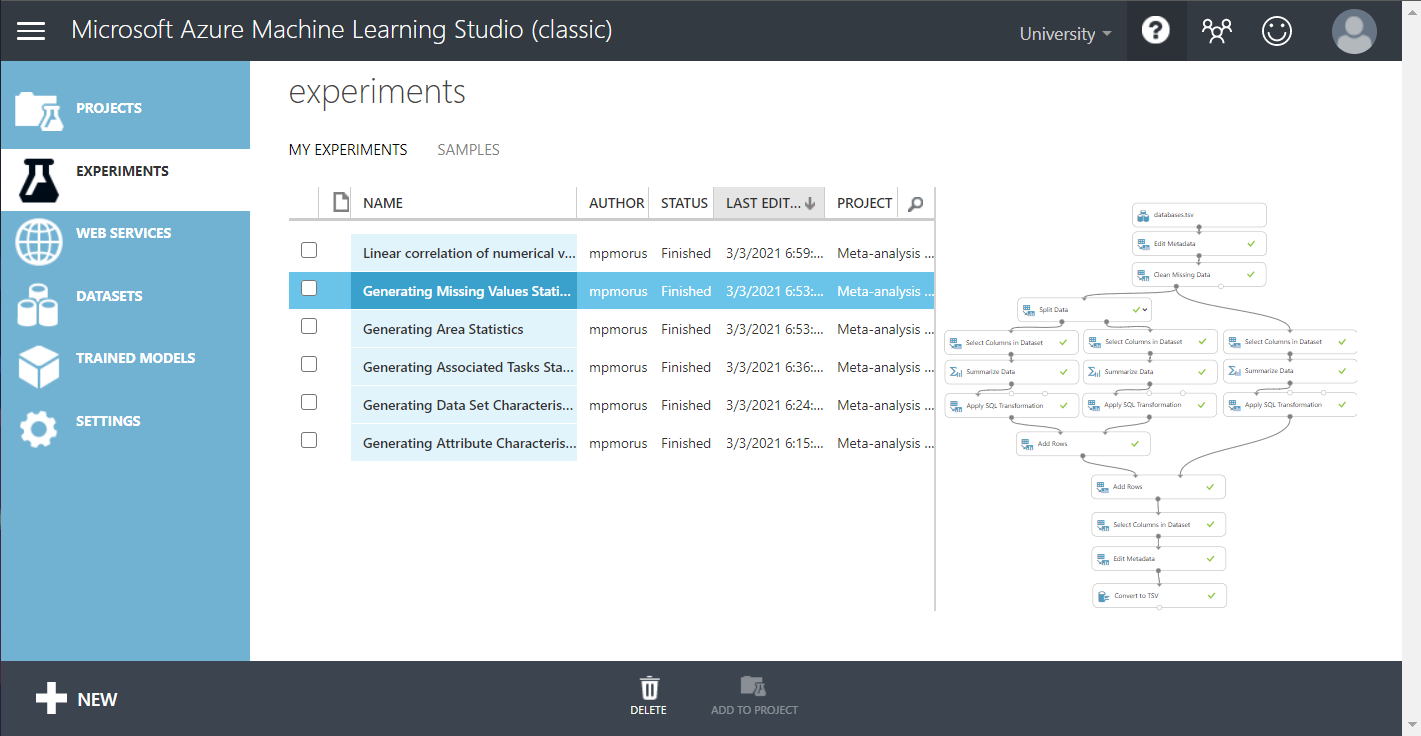
\includegraphics[width=\textwidth]{AzureML_interface}
	\caption{Interfejs programu Microsoft Azure Machine Learning Studio (classic)}
\end{figure}

Microsoft Azure Machine Learning Studio (dalej \emph{Azure ML}) to platforma stworzona przez firmę Microsoft oferująca interaktywną, wizualną przestrzeń roboczą przeznaczoną do tworzenia, testowania i wdrażania predykcyjnych modeli analitycznych.
Jest to aplikacja webowa działająca w przeglądarce, na celu mająca tworzenie modeli uczenia maszynowego.
Mimo to sprawdza się znakomicie jako narzędzie do samej analizy, pozwalając na stopniową obróbkę danych oraz ich wizualizację i przeglądanie na każdym kolejnym kroku.

Platforma oferuje możliwość importu i eksportu \emph{zbiorów danych} do obszaru roboczego, w którym pracujemy.
Podobnie można zapisywać i zarządzać wytrenowanymi \emph{modelami} klasyfikatorów.
Tworzenie \emph{projektów} pozwala na organizację zapisanych zbiorów danych, modeli i eksperymentów w zbiory tematycznie ze sobą powiązane.
Te ostatnie są najistotniejszym elementem platformy, w którym mieści się cała analiza danych, ich przetwarzanie i trenowanie modeli.

\emph{Eksperyment} w Azure ML to odrębny, kompletny obiekt przepływu informacji z wbudowanymi wszystkimi komponentami potrzebnymi do tworzenia, testowania i ewaluacji modeli predykcyjnych.
W eksperymencie moduły (komponenty) połączone są ze sobą liniami wskazującymi przepływ informacji i parametrów z wyjścia jednego do wejścia drugiego \cite{barga2015introducing}.

\begin{figure}[ht]
	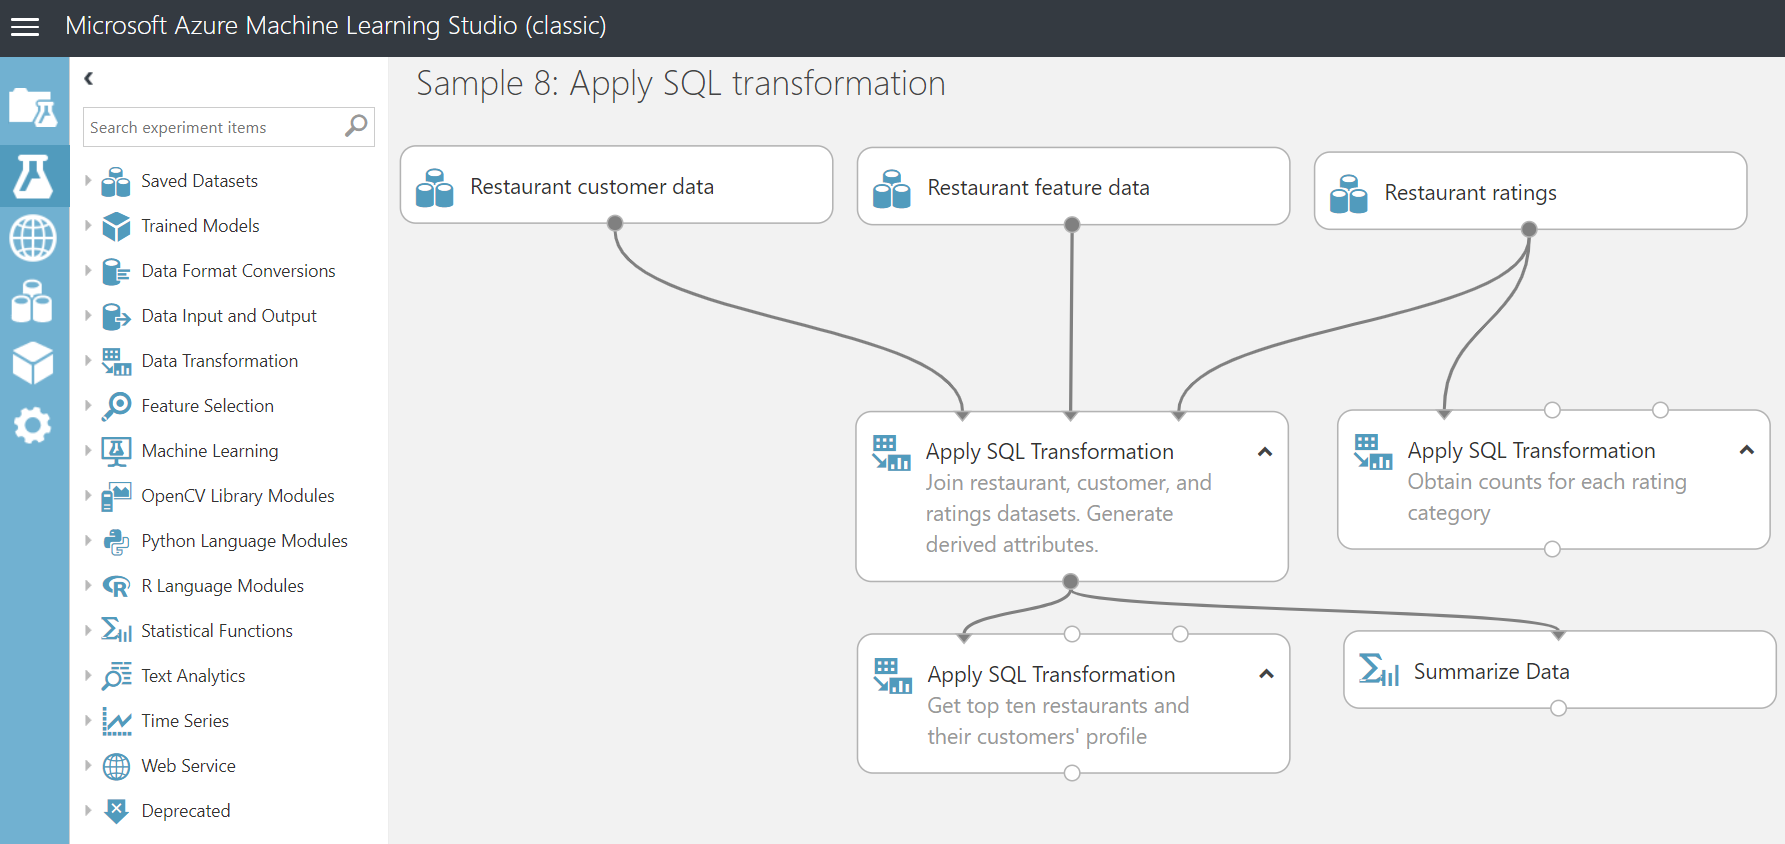
\includegraphics[width=\textwidth]{AzureML_experiment.png}
	\caption{Przykładowy schemat blokowy eksperymentu. Ten eksperyment przedstawia zastosowanie transformacji SQL na zbiorze danych wejściowych.}
\end{figure}


% Include the third chapter
\chapter{Badanie i projekt}

W niniejszej pracy przeprowadziłem metaanalizę na zbiorze danych pozyskanych z repozytorium zbiorów danych do uczenia maszynowego UCI \cite{Dua:2021}.
Większość kroków w badaniu (poza pozyskaniem danych) jest uniwersalnych i można je zastosować dla innych zbiorów danych o podobnej zawartości.

\section{Badanie}

Przeprowadzone badanie to analiza metadanych o zbiorach danych zawartych w repozytorium UCI \cite{Dua:2021}.
Serwis ten posiada informacje na temat wielu przekazanych im zbiorów danych, rejestrując jawnie informacje o ich cechach.
Cechy te to:

\begin{itemize}
  \item Cechy zbioru danych (\emph{Data Set Characteristics})
        Zawiera informacje o charakterystyce danego zbioru danych.
        Pojawia się tam, czy zbiór jest wielowymiarowy (\emph{Multivariate}), czy jednowymiarowy (\emph{Univariate}) \footnotemark.
        \footnotetext{Statystyka wielowymiarowa zajmuje się badaniem i obserwacją wielu zmiennych wyjścia (metryk) na raz. Statystyka jednowymiarowa bada wyłącznie zachowanie jednej zmiennej w zbiorze.}
        Zawarte jest również, czy zbiór ma charakter tekstowy \emph{Text}, czy może są to dane szeregu czasowego (\emph{Time-Series}).

  \item Cechy atrybutów (\emph{Attribute Characteristics})
        Zawiera informacje na temat typów atrybutów danych w zbiorze.
        Sprecyzowane są trzy wartości: zawartość danych kategorialnych (\emph{Categorical}), liczb całkowitych (\emph{Integer}) oraz rzeczywistych (\emph{Real}).

  \item Powiązane zadania (\emph{Associated Tasks})
        Zawiera informacje na temat głównych zadań, dla których dany zbiór jest przeznaczony.
        Może być to klasyfikacja (\emph{Classification}), regresja (\emph{Regression}) czy odnajdywanie powiązań przyczynowych (\emph{Causal-Discovery}).

  \item Liczba instancji (\emph{Number of Instances})
        Ilość krotek (rekordów) danych zawartych w zbiorze.
        Jeśli zbiór ma postać tabelaryczną, będzie to ilość zawartych w nim wierszy.

  \item Liczba atrybutów (\emph{Number of Attributes})
        Ilość cech, na temat których w rekordach zawarte są dane.
        Jeśli zbiór ma postać tabelaryczną, będzie to ilość zawartych w nim kolumn.

  \item Brakujące wartości (\emph{Missing Values})
        Zawiera informację, czy w zbiorze danych pojawiają się brakujące wartości.

  \item Obszar (\emph{Area})
        Zawiera informację na temat przynależności zbioru danych do jednej z ogólnie pojętych dziedzin tematycznych.
        Najczęściej pojawiające się tu wartości to dziedzina społeczna (\emph{Social}), fizyka (\emph{Physical}), informatyka (\emph{Computer}) oraz życie (\emph{Life}).

  \item Data dotacji (\emph{Date Donated})
        Data przekazania zbioru danych przez jego właściciela czy autora administracji repozytorium UCI.

  \item Ilość wyświetleń (\emph{Number of Web Hits})
        Liczba wszystkich osób odwiedzających stronę zawierającą zbiór danych.

\end{itemize}

\subsection{Pozyskanie danych}

Repozytorium UCI nie posiada API pozwalającego na dostęp do zawartych w nim danych.
Aby uzyskać dane w nim zawarte napisałem więc w języku Python program typu Scraper.

Część ze zbiorów danych na stronie posiada sekcję \emph{Papers That Cite This Data Set}.
Pierwotnie Scraper miał liczyć wymienione tam prace i zapisać jako dodatkowy atrybut generowanego zbioru danych: liczbę cytacji (\emph{Number of Citations}).
Jak się okazuje, listowanie prac cytujących dany zbiór wykonywane było automatycznie z pomocą portalu \emph{Rexa.info}.
Niestety, portal ten już nie istnieje i bardzo trudno znaleźć o nim informacje.
Co jest jednak pewne, to że w wygenerowanym zbiorze danych ostatni rekord, który posiada przynajmniej jedną cytację, ma datę dotacji w roku 2002.
Najprawdopodobniej mniej więcej w tamtym okresie portal \emph{Rexa.info} przestał zbierać informacje na temat cytacji zbiorów danych zawartych w repozytorium.
Tak czy inaczej, atrybut ten zebrany w ten sposób - mimo, że bardzo atrakcyjny jako metryka metaanalizy - nie nadaje się do tego badania z powodu jego bardzo ograniczonego zasięgu.
Stąd w finalnej wersji zbioru danych został on pominięty.

Program Scrapera został podzielony na dwie części, pierwsza odpowiedzialna za pobranie odpowiednich danych z sieci i zapisanie ich do pliku, a druga za przetworzenie powstałego pliku i dodanie do niego dodatkowych kolumn przydatnych przy analizie.
Część pierwsza sama również działa dwuetapowo.
Najpierw pobiera ze strony \url{http://archive.ics.uci.edu/ml/datasets} listę linków do poszczególnych zbiorów danych i zapisuje ją do pliku.
Następnie wczytuje ten plik z listą linków i kolejno otwiera dane linki prowadzące do podstron konkretnych zbiorów danych, skąd pobiera szczegółowe informacje na temat tego zbioru.
Taki podział pozwala na ręczną ingerencję w linki pobrane ze strony głównej, co okazuje się w tym przypadku być przydatne.
Pierwotnie pobranych linków było dokładnie 559, jednak 5 z nich jest uszkodzonych.
Ręczne wyszukanie zbiorów danych o podanej nazwie w internecie pozwoliło na odnalezienie trzech z nich.
Po poprawieniu linków do nich prowadzących w pliku i usunięciu tych, których nie udało się odnaleźć, powstał plik zawierający dokładnie 557 linków do podstron zbiorów danych w repozytorium.
Taki poprawiony plik następnie druga część Scrapera wykorzystała do wygenerowania zbioru składającego się z informacji o tych właśnie 557 zbiorach danych.

Druga część Scrapera wzbogaca powstały zbiór danych w dwa dodatkowe atrybuty wyliczeniowe.
Pierwszym jest ilość dni, jaką dany zbiór jest dostępny w repozytorium (\emph{Days Available}).
Otrzymywany on jest poprzez obliczenie różnicy między datą uruchomienia Scrapera a datą dotacji zbioru do repozytorium.
Następnie z użyciem tego pola skrypt dodaje jeszcze jedną kolumnę zawierającą liczbę wyświetleń danego zbioru na dzień (\emph{Number of Web Hits per Day}) poprzez podzielenie liczby wyświetleń przez liczbę dni dostępności zbioru.

\subsection{Przeprowadzenie analizy}

Za metrykę zbioru danych, względem której przeprowadzam analizę, obrałem ilość wyświetleń danego zbioru na dzień.
Wartość ta jest znormalizowana czasowo, co pozwala na uwzględnienie jej jako odzwierciedlenia popularności zbioru.

Analiza została przeprowadzona z użyciem portalu \emph{Azure Machine Learning Studio (classic)}.
Utworzyłem 6 eksperymentów wykorzystujący wygenerowany przez Scrapera zbiór danych.
Jeden z eksperymentów bada zależności między atrybutami numerycznymi, a pozostałe 5 dzielą zbiór na podzbiory bazując na różnych danych kategorialnych oraz liczą statystyki związane z wyświetleniami dla każdego z nich.

W Azure ML moduł odpowiedzialny za badanie zależności przy kolumnach numerycznych bazuje na wyliczeniu współczynnika korelacji liniowej Pearsona.
Zestawia on atrybuty na zasadzie ``każdy z każdym'' i liczy korelację liniową między nimi.
W ten sposób powstaje macierz korelacji, która na przekątnej będzie miała wartości \( 1.0 \) (każdy atrybut zestawiony jest również ze sobą, jest to więc autokorelacja).
Współczynnik korelacji mieści się w przedziale domkniętym \( [-1, 1] \).
Wartość ujemna mówi, że gdy jeden atrybut rośnie, drugi maleje, a dodatnia, że oba atrybuty wspólnie rosną i maleją.
Dodatkowo wartość bezwzględna współczynnika opisuje, jak silna jest zależność pomiędzy atrybutami.

5 pozostałych eksperymentów badało wpływ danych kategorialnych na obraną metrykę zbioru.
W każdym z nich zbiór został podzielony na kilka podzbiorów poprzez rozbicie jednej z kolumn kategorialnych na podkategorie, a następnie wyliczenie podstawowych statystyk numerycznych kolumny z metryką każdego z nich.
Przeprowadzone eksperymenty objęły podziałów ze względu na:

\begin{itemize}
  \item Charakterystykę zbioru danych (\emph{Data Set Characteristics})
        W tej kolumnie znajdowało się 12 unikatowych charakterystyk.
        Każdy rekord mógł posiadał wiele z nich oddzielonych przecinkami.
        Przynależność do podzbioru określałem poprzez obecność słowa kluczowego w tym atrybucie.
        Za granicę przyjęcia podzbioru do analizy ustaliłem, że musi posiadać przynajmniej 10 elementów.

  \item Charakterystykę atrybutów zbioru (\emph{Attribute Characteristics})
        W tej kolumnie znajdowały się dokładnie 3 unikatowe charakterystyki niewykluczające się wzajemnie.
        Stąd powstały 3 podzbiory na podobnej zasadzie jak wyżej.

  \item Obecność brakujących danych (\emph{Missing Values})
        Tutaj utworzone zostały dokładnie dwa podzbiory: zbiory zawierające brakujące dane oraz te ich nie zawierające.

  \item Powiązane zadania (\emph{Associated Tasks})
        W tej kolumnie znajdowało się 9 unikatowych, niewykluczających się wzajemnie zadań.
        Przynależność do podzbioru określałem analogicznie jak w eksperymencie z charakterystykami zbioru danych, podobnie za granicę dolną przyjmując 10 elementów podzbioru.

  \item Obszar (\emph{Area})
        Obszar cyberbezpieczeństwa (\emph{Computer Security}) zaliczyłem do obszaru informatyki, a finansowy (\emph{Financial}) do danych biznesowych.
        Te obszary znacznie rzadziej pojawiały się w uzyskanych danych (kolejno jednorazowo i 5 razy) i ich analiza nie była możliwa a dostępne były bliskie im szersze obszary.
        Obszar gier (\emph{Games}) również był ubogi (10 instancji) jednak nie przypasował się żadnej z większych dziedzin, stąd wykluczyłem go z analizy.

\end{itemize}

% Mediana lepsza niż średnia

\section{Wyniki}

Tabela \ref{tab:correlation} przedstawia macierz korelacji atrybutów numerycznych zbioru.
Oprócz trywialnej autokorelacji nie pojawia się nigdzie żadna silna zależność.
Najwyższa wartość ( \( \sim 0.13 \) ) występuje pomiędzy ilością instancji w zbiorze a obraną metryką liczby wyświetleń na dzień.
Najniższa z kolei ( \( \sim -0.02 \) ) zachodzi między wyświetleniami a ilością atrybutów.
Sugerowało by to, większa liczba instancji w zbiorze zwiększa jego popularność, natomiast liczba atrybutów na nią nie wpływa.
Ma to intuicyjny sens jednak jest korelacja bardzo niska, tym bardziej biorąc pod uwagę stosunkowo niewielką ilość instancji w zbiorze danych.
Tym samym generalizacje na niej bazujące będą przynajmniej niepewne, a prawdopodobnie również niepoprawne.
Nie można więc w tym wypadku wyciągnąć definitywnych konkluzji dotyczących tych atrybutów.

\begin{center}
  \begin{table}[ht]
    \begin{tabular}{|l|rrr|}
      \hline
                           & Number of Instances & Number of Attributes & Web Hits per Day \\
      \hline
      Number of Instances  & 1                   & 0.099287             & 0.126046         \\
      Number of Attributes & 0.099287            & 1                    & -0.024657        \\
      Web Hits per Day     & 0.126046            & -0.024657            & 1                \\
      \hline
    \end{tabular}
    \caption{Macierz korelacji liniowej między wartościami numerycznymi w zbiorze danych}
    \label{tab:correlation}
  \end{table}
\end{center}

Znacznie więcej informacji przynosi analiza zbiorów danych przy podziale atrybutów kategorialnych.
Analiza charakterystyk zbiorów danych (rysunek \ref{fig:datasetcharacteristics}) pokazuje, że najbardziej użyteczne zbiory danych zawierają szeregi czasowe (\emph{Time-Series}).
Co ciekawe, dane tekstowe są raczej mniej popularne.
Z kolei zbiory zawierające dane domenowe (\emph{Domain-Theory}) otrzymują wyraźnie najmniej zainteresowania.
Dane jednowymiarowe są również popularniejsze niż wielowymiarowe, chociaż tutaj różnica jest znacznie mniejsza.

\begin{figure}[ht]
  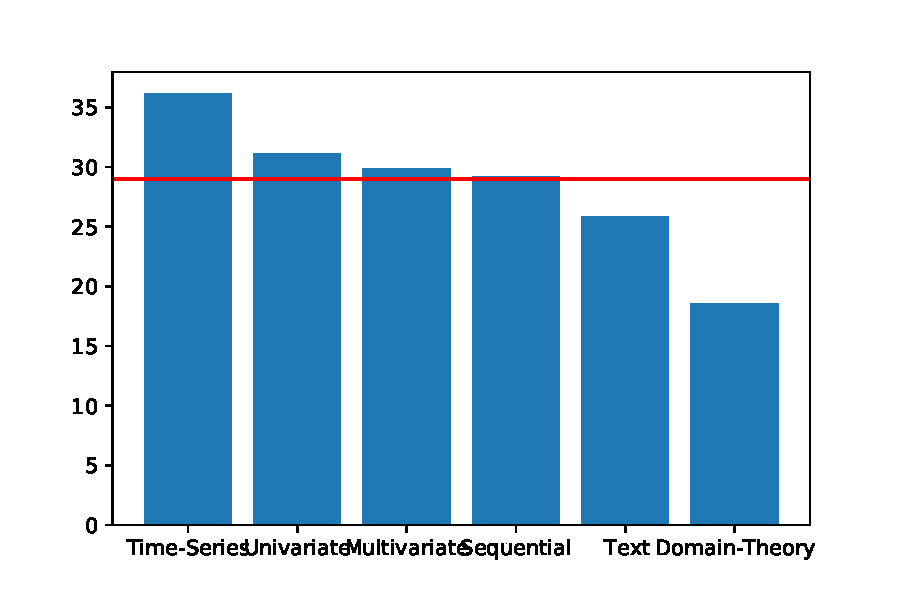
\includegraphics[width=\textwidth]{DataSetCharacteristics}
  \caption{Analiza mediany liczby dziennych wyświetleń zbiorów danych względem ich charakterystyki}
  \label{fig:datasetcharacteristics}
\end{figure}

Analiza rodzaju danych atrybutów zawartych w zbiorach (rysunek \ref{fig:attributecharacteristics}) pokazuje, że największym zainteresowaniem cieszą się zbiory zawierające wartości rzeczywiste.
Zawieranie liczb całkowitych jest blisko mediany ogólnej, co mówi, że ogólnie dane liczbowe są preferowane.
Dane kategorialne bowiem znacznie odbiegają od reszty i są zdecydowanie mniej popularne.

\begin{figure}[ht]
  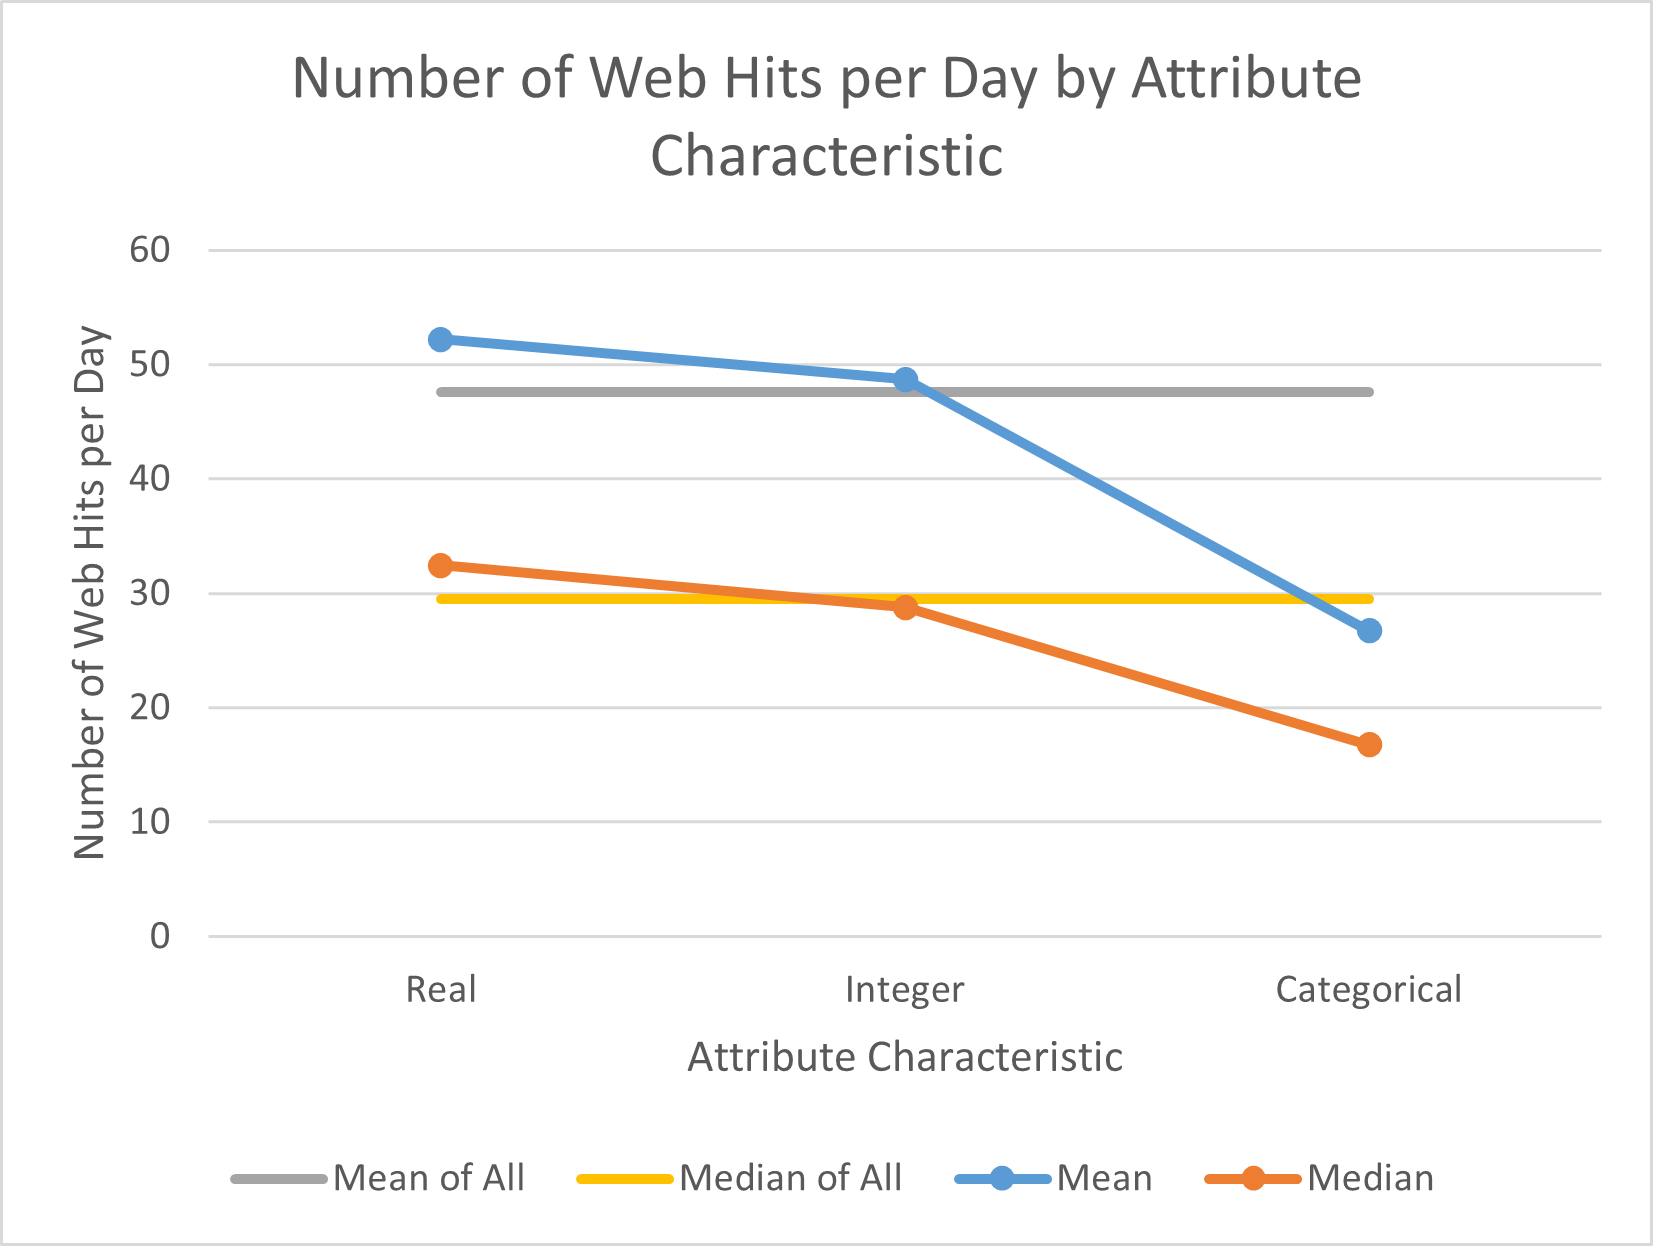
\includegraphics[width=\textwidth]{AttributeCharacteristics}
  \caption{Analiza mediany liczby dziennych wyświetleń zbiorów danych względem charakterystyki zawartych w nich danych}
  \label{fig:attributecharacteristics}
\end{figure}

Przy analizie powiązanych zadań (rysunek \ref{fig:associatedtasks}) również można wyciągnąć dość wyraźne wnioski.
Najpopularniejsze są zbiory danych przeznaczone do przeprowadzania na nich regresji (\emph{Regression}), a tuż za nimi te przeznaczone do analizy skupień (\emph{Clustering}).
Zbiory powiązane z klasyfikacją (\emph{Classification}) nie odbiegają od normy, a najmniejszym zainteresowaniem cieszą się te związane z analizą przyczynową (\emph{Causal-Discovery}).

\begin{figure}[ht]
  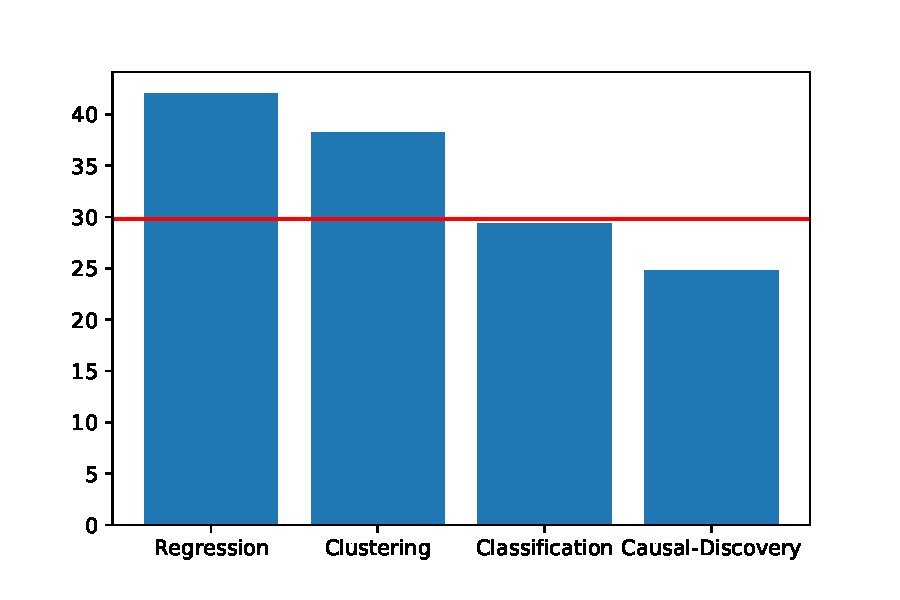
\includegraphics[width=\textwidth]{AssociatedTasks}
  \caption{Analiza mediany liczby dziennych wyświetleń zbiorów danych względem powiązanych z nimi zadań}
  \label{fig:associatedtasks}
\end{figure}

Analizując bardziej semantyczną zawartość zbiorów danych, czyli ogólny obszar ich pochodzenia (rysunek \ref{fig:area}) widać, że wyraźnie najpopularniejsze są zbiory zawierające dane biznesowe.
Średnia wyświetleń zbiorów z dziedziny społecznej również wykracza poza średnią ogólną, chociaż ich mediana już takiej tendencji nie wykazuje.
Biorąc pod uwagę ten fakt i naturę relacji między średnią a medianą można wyciągnąć wniosek, że w tym obszarze kilka najczęściej odwiedzanych zbiorów mocno wybiega popularnością poza pozostałe.
95. percentyl jest równy \(215.98\), co jest prawie najwyższą wartością, jedynie za biznesem (\(303.41\)).
Z kolei 5. percentyl nie odbiega mocno od pozostałych.
W odwrotnej sytuacji są zbiory informatyczne, których 95. percentyl wynosi zaledwie \(98.93\), tylko \(75\%\) następnej najniższej wartości (obszaru fizyki).
Ta grupa ma z kolei sporo zbiorów wyjątkowo mało popularnych.
Jednak ich mediana również się nie wyróżnia.
Jedyną grupą wyróżniającą się z innych poza biznesową jest fizyczna.
Są one mniej popularne zarówno patrząc na średnią, jak i medianę podzbioru.

\begin{figure}[ht]
  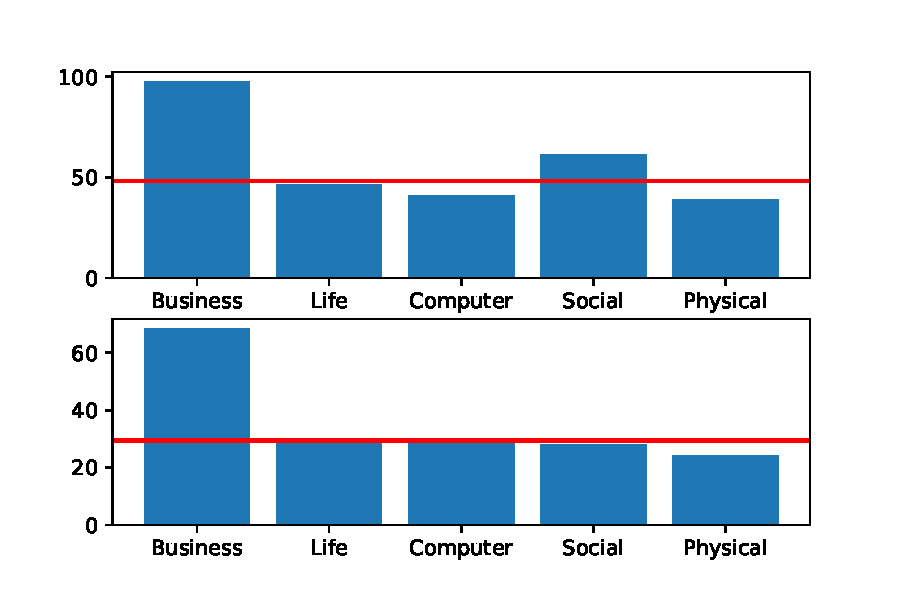
\includegraphics[width=\textwidth]{Area}
  \caption{Analiza mediany i średniej liczby dziennych wyświetleń zbiorów danych względem ich dziedziny}
  \label{fig:area}
\end{figure}

Ciekawą sytuację przedstawia analiza brakujących danych przedstawiona na rysunku \ref{fig:missingvalues}.
Sugeruje ona, że zbiory posiadające brakujące dane przyciągają więcej osób niż te, które ich nie mają.
Jest to sprzeczne z tym, czego można by się spodziewać zarówno intuicyjnie, jak i biorąc pod uwagę ocenę jakości zbiorów danych.
Można to jednak wytłumaczyć biorąc pod uwagę inne cechy zbiorów.
Biorąc pod uwagę szeregi czasowe, najpopularniejszy rodzaj danych, 27 z 32 rekordów zawierających na ten temat informacje posiada brakujące dane (\(~84\%\).
Z kolei najmniej popularne dane domenowe wykazują odwrotną tendencję, gdzie \(75\%\) z nich nie zawiera brakujących danych.

Podobna sytuacja ma miejsce gdy weźmiemy pod uwagę rodzaj atrybutów.
Zdecydowanie najpopularniejsze zbiory zawierające liczby rzeczywiste posiadają brakujące dane w \(~72\%\) przypadków (71 z 98), a najmniej pożądane dane kategorialne odwrotnie, nie posiadają brakujących danych w \(55\%\) przypadków (40 z 73).
Najpopularniejszy rodzaj docelowego przeznaczenia, regresja, także wykazuje ponadprzeciętną zawartość brakujących danych (34 z 39, czyli \(~87\%\)).

Jak widać to popularniejsze kategorie danych mają dużą zawartość brakujących danych, natomiast mniej popularne mają ich znacznie mniej.
Wynikać to może z natury charakterystyk popularniejszych zbiorów danych, które z założenia posiadają więcej braków, jednak są one mało istotne z perspektywy użyteczności.
Jest również możliwość, że istniejące algorytmy uzupełniania brakujących danych takie jak MICE czy PCA są na tyle dobre, że nieduże ubytki nie wpływają na jakoś uczenia czy analizy.
Tłumaczyłoby to w szczególności różnicę między wpływem brakujących danych na liczby rzeczywiste, a dane kategorialne, jako, że dane liczbowe można uzupełnić wspomnianymi wcześniej metodami.

\begin{figure}[ht]
  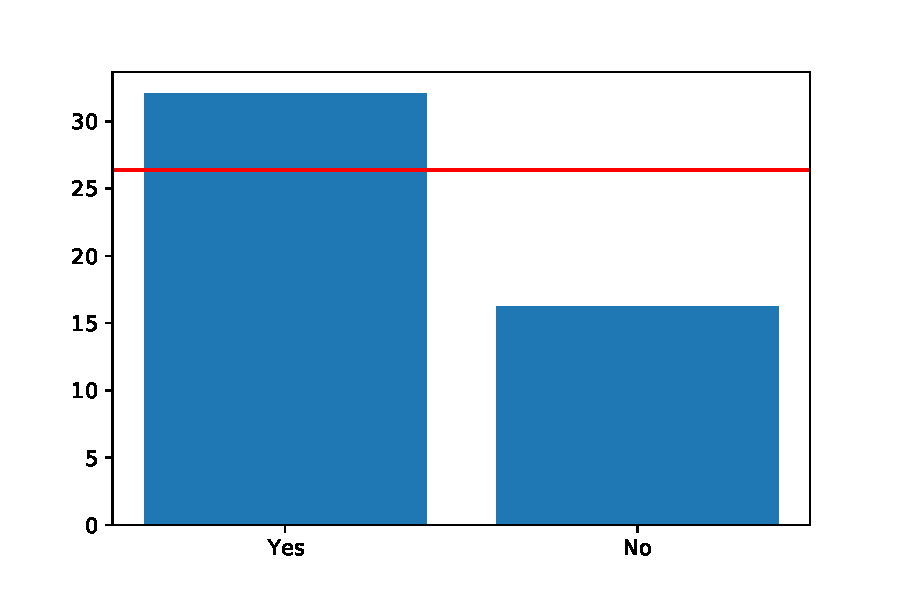
\includegraphics[width=\textwidth]{MissingValues}
  \caption{Analiza mediany liczby dziennych wyświetleń zbiorów danych względem brakujących danych}
  \label{fig:missingvalues}
\end{figure}

\section{Dyskusja}


% Add the Bibliography to the contents page
\addcontentsline{toc}{chapter}{Bibliografia}
% Use a bibtex bibliography file refs.bib
\bibliography{refs}
% Use the plain bibliography style ordered by citation
\bibliographystyle{unsrt}

\end{document}
